\documentclass[10pt]{article}
% header.tex
% this is where you load pacakges, specify custom formats, etc.

\usepackage[margin=1in,footskip=25pt]{geometry} 
% \usepackage{changepage}
\usepackage{amsmath,amsthm,amssymb,amsfonts,bbm}
\usepackage{mathtools}
% enumitem for custom lists
\usepackage{enumitem}
% Load dsfont this to get proper indicator function (bold 1) with \mathds{1}:
\usepackage{dsfont}
\usepackage{centernot}

\usepackage[usenames,dvipsnames]{xcolor}

% set up commenting code (I will use this during marking)
\definecolor{CommentColor}{rgb}{0,.50,.50}
\newcounter{margincounter}
\newcommand{\displaycounter}{{\arabic{margincounter}}}
\newcommand{\incdisplaycounter}{{\stepcounter{margincounter}\arabic{margincounter}}}
\newcommand{\COMMENT}[1]{\textcolor{CommentColor}{$\,^{(\incdisplaycounter)}$}\marginpar{\scriptsize\textcolor{CommentColor}{ {\tiny $(\displaycounter)$} #1}}}

\usepackage{appendix}

% set up graphics
\usepackage{graphicx}
\DeclareGraphicsExtensions{.pdf,.png,.jpg}
\graphicspath{ {fig/} }

\usepackage{fancyhdr}
\pagestyle{fancy}
\setlength{\headheight}{40pt}


\usepackage[numbers,sort]{natbib}

%%%%%%%%%%%%%%%%%%%%%%%%%%%%%%%%%%%%%%%%%%%%%%%%%%%%%%%%%%%%%%%%%%%%%%%%%%%%%%%%%%%%
% most other packages you might use should be loaded before hyperref
%%%%%%%%%%%%%%%%%%%%%%%%%%%%%%%%%%%%%%%%%%%%%%%%%%%%%%%%%%%%%%%%%%%%%%%%%%%%%%%%%%%%

% Set up hyperlinks:
\definecolor{RefColor}{rgb}{0,0,.65}
\usepackage[colorlinks,linkcolor=RefColor,citecolor=RefColor,urlcolor=RefColor]{hyperref}

\usepackage[capitalize]{cleveref}
\crefname{appsec}{Appendix}{Appendices} % you can tell cleveref what to call things
% defs.tex
% this is where you define custom notation, commands, etc.


%%
% full alphabets of different styles
%%

% bf series
\def\bfA{\mathbf{A}}
\def\bfB{\mathbf{B}}
\def\bfC{\mathbf{C}}
\def\bfD{\mathbf{D}}
\def\bfE{\mathbf{E}}
\def\bfF{\mathbf{F}}
\def\bfG{\mathbf{G}}
\def\bfH{\mathbf{H}}
\def\bfI{\mathbf{I}}
\def\bfJ{\mathbf{J}}
\def\bfK{\mathbf{K}}
\def\bfL{\mathbf{L}}
\def\bfM{\mathbf{M}}
\def\bfN{\mathbf{N}}
\def\bfO{\mathbf{O}}
\def\bfP{\mathbf{P}}
\def\bfQ{\mathbf{Q}}
\def\bfR{\mathbf{R}}
\def\bfS{\mathbf{S}}
\def\bfT{\mathbf{T}}
\def\bfU{\mathbf{U}}
\def\bfV{\mathbf{V}}
\def\bfW{\mathbf{W}}
\def\bfX{\mathbf{X}}
\def\bfY{\mathbf{Y}}
\def\bfZ{\mathbf{Z}}

% bb series
\def\bbA{\mathbb{A}}
\def\bbB{\mathbb{B}}
\def\bbC{\mathbb{C}}
\def\bbD{\mathbb{D}}
\def\bbE{\mathbb{E}}
\def\bbF{\mathbb{F}}
\def\bbG{\mathbb{G}}
\def\bbH{\mathbb{H}}
\def\bbI{\mathbb{I}}
\def\bbJ{\mathbb{J}}
\def\bbK{\mathbb{K}}
\def\bbL{\mathbb{L}}
\def\bbM{\mathbb{M}}
\def\bbN{\mathbb{N}}
\def\bbO{\mathbb{O}}
\def\bbP{\mathbb{P}}
\def\bbQ{\mathbb{Q}}
\def\bbR{\mathbb{R}}
\def\bbS{\mathbb{S}}
\def\bbT{\mathbb{T}}
\def\bbU{\mathbb{U}}
\def\bbV{\mathbb{V}}
\def\bbW{\mathbb{W}}
\def\bbX{\mathbb{X}}
\def\bbY{\mathbb{Y}}
\def\bbZ{\mathbb{Z}}

% cal series
\def\calA{\mathcal{A}}
\def\calB{\mathcal{B}}
\def\calC{\mathcal{C}}
\def\calD{\mathcal{D}}
\def\calE{\mathcal{E}}
\def\calF{\mathcal{F}}
\def\calG{\mathcal{G}}
\def\calH{\mathcal{H}}
\def\calI{\mathcal{I}}
\def\calJ{\mathcal{J}}
\def\calK{\mathcal{K}}
\def\calL{\mathcal{L}}
\def\calM{\mathcal{M}}
\def\calN{\mathcal{N}}
\def\calO{\mathcal{O}}
\def\calP{\mathcal{P}}
\def\calQ{\mathcal{Q}}
\def\calR{\mathcal{R}}
\def\calS{\mathcal{S}}
\def\calT{\mathcal{T}}
\def\calU{\mathcal{U}}
\def\calV{\mathcal{V}}
\def\calW{\mathcal{W}}
\def\calX{\mathcal{X}}
\def\calY{\mathcal{Y}}
\def\calZ{\mathcal{Z}}


%%%%%%%%%%%%%%%%%%%%%%%%%%%%%%%%%%%%%%%%%%%%%%%%%%%%%%%%%%
% text short-cuts
\def\iid{i.i.d.\ } %i.i.d.
\def\ie{i.e.\ }
\def\eg{e.g.\ }
\def\Polya{P\'{o}lya\ }
%%%%%%%%%%%%%%%%%%%%%%%%%%%%%%%%%%%%%%%%%%%%%%%%%%%%%%%%%%

%%%%%%%%%%%%%%%%%%%%%%%%%%%%%%%%%%%%%%%%%%%%%%%%%%%%%%%%%%
% quasi-universal probabilistic and mathematical notation
% my preferences (modulo publication conventions, and clashes like random vectors):
%   vectors: bold, lowercase
%   matrices: bold, uppercase
%   operators: blackboard (e.g., \mathbb{E}), uppercase
%   sets, spaces: calligraphic, uppercase
%   random variables: normal font, uppercase
%   deterministic quantities: normal font, lowercase
%%%%%%%%%%%%%%%%%%%%%%%%%%%%%%%%%%%%%%%%%%%%%%%%%%%%%%%%%%

% operators
\def\P{\bbP} %fundamental probability
\def\E{\bbE} %expectation

\newcommand{\Expect}[1]{\E \left{ #1\right}}
% conditional expectation
\DeclarePairedDelimiterX\bigCond[2]{[}{]}{#1 \;\delimsize\vert\; #2}
\newcommand{\conditional}[3][]{\E_{#1}\bigCond*{#2}{#3}}
\def\Law{\mathcal{L}} %law; this is by convention in the literature
\def\indicator{\mathds{1}} % indicator function

% norms
\newcommand{\norm}[1]{\left\lVert #1 \right\rVert}

% binary relations
\def\condind{{\perp\!\!\!\perp}} %independence/conditional independence
\def\equdist{\stackrel{\text{\rm\tiny d}}{=}} %equal in distribution
\def\equas{\stackrel{\text{\rm\tiny a.s.}}{=}} %euqal amost surely
\def\simiid{\sim_{\mbox{\tiny iid}}} %sampled i.i.d

% common vectors and matrices
\def\onevec{\mathbf{1}}
\def\iden{\mathbf{I}} % identity matrix
\def\supp{\text{\rm supp}}

% misc
% floor and ceiling
\DeclarePairedDelimiter{\ceilpair}{\lceil}{\rceil}
\DeclarePairedDelimiter{\floor}{\lfloor}{\rfloor}
\newcommand{\argdot}{{\,\vcenter{\hbox{\tiny$\bullet$}}\,}} %generic argument dot
%%%%%%%%%%%%%%%%%%%%%%%%%%%%%%%%%%%%%%%%%%%%%%%%%%%%%%%%%%

%%%%%%%%%%%%%%%%%%%%%%%%%%%%%%%%%%%%%%%%%%%%%%%%%%%%%%%%%%
%% some distributions
% continuous
\def\UnifDist{\text{\rm Unif}}
\def\BetaDist{\text{\rm Beta}}
\def\ExpDist{\text{\rm Exp}}
\def\GammaDist{\text{\rm Gamma}}
\def\NormalDist{\text{\rm Normal}}


% discrete
\def\BernDist{\text{\rm Bernoulli}}
\def\BinomDist{\text{\rm Binomial}}
\def\PoissonDist{\text{\rm Poisson}}
%%%%%%%%%%%%%%%%%%%%%%%%%%%%%%%%%%%%%%%%%%%%%%%%%%%%%%%%%%

%%%%%%%%%%%%%%%%%%%%%%%%%%%%%%%%%%%%%%%%%%%%%%%%%%%%%%%%%%
% Project-specific notation should go here
% (Because it's at the end of the file, it can overwrite anything that came before.)

\DeclareMathOperator*{\argmax}{arg\,max}
\DeclareMathOperator*{\argmin}{arg\,min}

\def\bfa{\mathbf{a}}
\def\bfb{\mathbf{b}}
\def\bfx{\mathbf{x}}
\def\bfy{\mathbf{y}}

\def\T{\top}

\def\esd{e.s.d.}
\def\lsd{l.s.d.}

\newtheorem{theorem}{Theorem}
\newtheorem{conjecture}[theorem]{Conjecture}

\theoremstyle{definition}
\newtheorem{definition}{Definition}
\newtheorem{assumption}[definition]{Assumption}

\def\todo{{\color{Red} TODO}}

%%%%%%%%%%%%%%%%%%%%%%%%%%%%%%%%%%%%%%%%%%%%%%%%%%%%%%%%%%


\title{A critical and theoretical analysis of\\unbiased implicit variational inference}
\author{Kenny Chiu}
\date{\today}

\begin{document}

\maketitle


\newpage


\section{Critical analysis}

\subsection{Introduction}

\citet{Titsias:2019} introduce \textit{unbiased implicit variational inference} (\uivi) as a variational inference method with a flexible variational family and that addresses the issues of the existing methods that it is built on. In this analysis, we summarize the work of \citet{Titsias:2019} in the context of the literature and discuss the strengths and limitations of \uivi. This analysis is organized as follows: Section~\ref{an:literature} introduces the problem context and previous work; Section~\ref{an:uivi} describes how \uivi works, how it addresses the limitations of previous methods, and its own limitations; and Section~\ref{an:postpaper} highlights related work in the recent literature and discusses the general direction that the literature is moving towards.

\subsection{Context and previous work} \label{an:literature}

Variational inference (\vi) \citep{Jordan:1999} is a Bayesian inference method that formulates the problem of finding the posterior distribution $p(\bfz|\bfx)$ of latent variables $\bfz$ given data $\bfx$ as an optimization problem. \vi posits a variational family $\calQ=\{q_\theta\}$ of distributions indexed by variational parameters $\theta$, and the goal is to identify the variational distribution $q_\theta(\bfz)\in\calQ$ that best approximates the posterior distribution. In standard \vi, the selected distribution $q_\theta$ is the one that minimizes the Kullback-Leibler (\kl) divergence of $q_\theta$ and $p(\bfz|\bfx)$, or equivalently, the one that maximizes the evidence lower bound (\elbo) denoted as
\[
\calL(\theta) = \E_{q_\theta(\bfz)}\left[\log p(\bfx,\bfz) - \log q_\theta(\bfz)\right] \;.
\]
Standard \vi maximizes the \elbo using a coordinate ascent algorithm, which requires placing strong restrictions on the choice of the model and the variational family. These restrictions include (1) a mean-field assumption where the latent variables $\bfz$ are marginally independent and the variational distribution factorizes as $q_\theta(\bfz)=\prod_{i=1}^dq_{\theta_i}(\bfz_i)$, and (2) the model has conjugate conditionals where $p(\bfz_i)$ and $p(\bfz_i|\bfx,\bfz_{\neg i})$ are from the same distribution family. These assumptions implied that the choice of a variational family were often limited to analytical, exponential families and that marginal dependencies could not be modeled.
\\

An important development after standard \vi was black box \vi (\bbvi) \citep{Ranganath:2014}, which relaxed the restrictive assumptions by optimizing the \elbo using a different approach. By rewriting the \elbo gradient in terms of an expectation, the gradient could be estimated unbiasedly and cheaply using Monte Carlo samples. The optimization approach of \bbvi exchanges the restrictive assumptions of standard \vi for the different assumption that one can sample from the variational distribution $q_\theta(\bfz)$. This expanded the possibilities for the choice of the variational family. One such proposed family was the hierarchical variational model (\hvm) \citep{Ranganath:2016} containing distributions of the form $q_\theta(\bfz) = \int q_\theta(\bfz|\bfeps)q_\theta(\bfeps)d\bfeps$. An advantage of these hierarchical distributions over other variational distributions is the ease in being able to capture marginal dependencies between latent variables through the mixing distribution $q_\theta(\bfeps)$.
\\

Further pushing the assumption that one only needs to be able to sample from the variational distribution, one trend following the introduction of the \hvm was the incorporation of deep neural networks to expand the modeling capacity of the hierarchical variational family. These models took various forms, such as through normalizing flows~\citep{Rezende:2015} or through implicit distributions~\citep{Mohamed:2016} involving deep networks in which the density cannot be evaluated. Though the implicit models are flexible, the log density ratio in the \elbo is intractable in these models. Some works proposed using density ratio estimation to tackle this problem~\citep[e.g.,][]{Mohamed:2016,Huszar:2017}, but this approach is known to struggle in high-dimensional regimes~\citep{Sugiyama:2012}.
\\

The method that precedes \uivi and that was proposed to address the challenges of using implicit distributions in hierarchical variational models is \textit{semi-implicit} \vi (\sivi)~\citep{Yin:2018}. \textsc{Sivi} makes use of a semi-implicit variational distribution in which the variational conditional $q_\theta(\bfz|\bfeps)=q(\bfz|\bfeps)$ is required to be reparameterizable~\citep{Kingma:2013} and explicit while the mixing distribution $q_\theta(\bfeps)$ is required to be also reparameterizable but possibly implicit. \textsc{Sivi} then avoids the density ratio estimation problem by instead optimizing a lower bound for the \elbo that is only exact as the number of samples in each iteration goes to infinity~\citep{Yin:2018,Molchanov:2019}.


\subsection{Current work} \label{an:uivi}

\citet{Titsias:2019} propose \uivi as an alternative to \sivi that directly maximizes the \elbo as an objective rather than a surrogate lower bound. The motivation for \uivi is that directly optimizing the \elbo objective should be more efficient than optimizing a surrogate and therefore should result in faster convergence to the optimal variational approximation. \textsc{Uivi} allows for an \elbo objective by rewriting the \elbo gradient in terms of two expectations. One expectation is easily estimated using Monte Carlo samples, while the other expectation is over an inverse conditional from which \uivi draws samples using Markov chain Monte Carlo (\mcmc) methods.

\subsubsection{Unbiased implicit variational inference}

Like in \sivi, \uivi starts with a hierarchical variational model setup where the variational distribution is
\[
q_\theta(\bfz) = \int q_\theta(\bfz|\bfeps)q(\bfeps)d\bfeps \;.
\]
\textsc{Uivi} requires the variational conditional $q_\theta(\bfz|\bfeps)$ to be reparameterizable, i.e., that any sample $\bfz\sim q_\theta(\bfz|\bfeps)$ can be rewritten as
\[
\bfz = h_\theta(\bfu;\bfeps) := h_{\bfpsi=g_\theta(\bfeps)}(\bfu) 
\]
where $h_{\bfpsi}$ is some reparameterization function with parameters $\bfpsi$ that are the output of some arbitrarily complex function $g_\theta$ that depends on variational parameters $\theta$ and input $\bfeps$. To sample from $q_\theta(\bfz)$, noise variables $\bfu\sim q(\bfu)$ and $\bfeps\sim q(\bfeps)$ are first sampled from fixed auxiliary distributions and then fed through $h_\theta$. \textsc{Uivi} also requires that $q_\theta(\bfz|\bfeps)$ and its log-gradient $\nabla_\bfz\log q_\theta(\bfz|\bfeps)$ can be evaluated, which holds for common reparameterizable distributions such as Gaussian.
\\

Under these assumptions, the \elbo can be rewritten as an expectation with respect to the noise distributions $q(\bfu)$ and $q(\bfeps)$ through a change of variables, and its gradient can be decomposed into two expectation terms given by
\[
\nabla_\theta \calL(\theta) = \E_{q(\bfeps)q(\bfu)}\left[\nabla_\bfz \log p(\bfx,\bfz)\big|_{\bfz=h_\theta(\bfu;\bfeps)}\nabla_\theta h_\theta(\bfu;\bfeps)\right] - \E_{q(\bfeps)q(\bfu)}\left[\nabla_\bfz \log q_\theta(\bfz)\big|_{\bfz=h_\theta(\bfu;\bfeps)}\nabla_\theta h_\theta(\bfu;\bfeps)\right] \;.
\]
The first expectation can be estimated using samples from $q(\bfeps)$ and $q(\bfu)$ while the second expectation is more difficult as $\nabla_\bfz\log q_\theta(\bfz)$ may not be computable if $q_\theta(\bfz)$ is implicit. The first key trick in \uivi is to rewrite the gradient in the second term as an expectation given by
\[
\nabla_z\log q(\bfz) = \E_{q_\theta(\bfeps|\bfz)}\left[\nabla_\bfz\log q_\theta(\bfz|\bfeps)\right]
\]
which then allows for Monte Carlo estimation using samples from $q_\theta(\bfeps|\bfz)\propto q_\theta(\bfz|\bfeps)q(\bfeps)$. A \mcmc sampler is used to sample from $q_\theta(\bfeps|\bfz)$, and the second key trick in \uivi is to reuse the sample $(\bfz_i,\bfeps_i)$ used to estimate the outer expectation as an initial point in the \mcmc sampler. As the initial point is a sample from the same joint distribution $q_\theta(\bfz,\bfeps)$, no burn-in is necessary and the only purpose of the \mcmc is to break the dependence between samples used to estimate the inner and outer expectations. Thus, the gradient of the \elbo is estimated by
\[
\widehat{\nabla}_\theta\calL(\theta) = \frac{1}{n}\sum_{i=1}^n \left(\nabla_\bfz\log p(\bfx,\bfz)\big|_{\bfz=h_\theta(\bfu_i;\bfeps_i)} - \frac{1}{m}\sum_{j=1}^m \nabla_\bfz\log q_\theta(\bfz|\bfeps_j')\big|_{\bfz=h_\theta(\bfu_i;\bfeps_i)} \right)\nabla_\theta h_\theta(\bfu_i;\bfeps_i)
\]
where $\bfeps_i\sim q(\bfeps)$, $\bfu_i\sim q(\bfu)$, $\bfeps_j'\sim q_\theta(\bfeps|\bfz)$ and with $n=1$, $m=5$ said to be used in practice.

\subsubsection{Other contributions}

Aside from the \uivi algorithm, other contributions of the paper by \citet{Titsias:2019} include the empirical evaluations of \uivi on synthetic and benchmark datasets. Using a Gaussian conditional with a neural network for the mean parameter, Hamiltonian Monte Carlo (\hmc) for the \mcmc estimation of the \elbo gradient, and otherwise a fairly standard setup, \uivi is shown to be able to visually approximate various synthetic 2D distributions. Under a similar setup, \uivi is shown to be able to achieve better predictive performance than \sivi on the MNIST and HAPT~\citep{Reyes:2014} datasets while being comparable in terms of time per iteration. Finally, \citet{Titsias:2019} show that for a variational autoencoder (\vae)~\citep{Kingma:2013} with a semi-implicit variational distribution, \uivi achieves a greater marginal log-likelihood on the test set compared to standard \vae and \sivi on the MNIST and Fashion-MNIST datasets.

\subsubsection{Limitations}

The paper by \citet{Titsias:2019} has a few limitations. The main limitation is the lack of theoretical guarantees for the performance and convergence of \uivi. For example, it is unclear what the modeling capabilities are for the \uivi variational family, and no guidance is given on how to construct the model such that the true posterior is in or at least well-approximated by a member of the variational family. It is also unclear how good of an approximation \uivi is able to guarantee through its optimization procedure. However, we recognize that this is a common problem across the \vi literature and generally stems from the challenge of analyzing general purpose methods that may include intractable and non-analytic components.
\\

Another notable limitation of the paper is the missing discussion of the limitations of \uivi. In particular, the showcased experiments do not stress test \uivi, and there is no mention of future directions for improving or extending \uivi. Related work published after the paper by \citet{Titsias:2019} reported limited scalability with the number of latent parameters~\citep{Molchanova:2019,Moens:2021}. This is likely a consequence of the stochastic optimization of the \elbo as well as the use of \mcmc, both for which require an increasing number of samples to maintain estimation quality in response to an increasing number of dimensions. The \mcmc sampling in the \uivi optimization procedure may also result in greater variance of the \elbo gradient estimates~\citep{Betancourt:2015} and further contribute to non-scalability by complicating potential parallelization of the algorithm~\citep{Sobolev:2019}. In some instances, other issues common to \mcmc approaches, such as poor mixing over different modes, appear to inhibit the performance of \uivi~\citep{Sobolev:2019}. \todo gaussian interpretation


\subsection{Other related work} \label{an:postpaper}

While \uivi was proposed as an improved alternative to \sivi, there does not appear to be follow-up work in the literature that directly extends \uivi. As mentioned in the previous section, the inefficiency of \mcmc in high-dimensional regimes is often cited as the main problem of \uivi~\citep{Molchanova:2019,Moens:2021}. It appears that rather than trying to address this issue in \uivi, recent work in the literature return to \sivi and propose methods that either improve the quality of its approximation or allow it to scale more efficiently to high dimensions.
\\

Several strategies for improving the \sivi approximation have been proposed in the literature around the time of or after the work by \citet{Titsias:2019}. \citet{Molchanov:2019} proposed \textit{doubly}~\sivi (\dsivi) that expands the flexibility of standard \sivi by allowing both the posterior and prior to be semi-implicit. \citet{Sobolev:2019} introduced \textit{importance weighted hierarchical}~\vi (\iwhvi), which optimizes a \sivi-like lower bound that incorporates elements from the bound used in importance weighted autoencoders~\citep{Burda:2015}. \textsc{Sivi}, \dsivi and \hvm can be seen as special cases of \iwhvi and so the bound in \iwhvi has the capacity to result in a tighter lower bound~\citep{Sobolev:2019}.
\\

Recent work in the literature have focused more on improving the scalability of \sivi to high dimensions. \citet{Molchanova:2019} proposed \textit{structured}~\sivi where the high-dimensional semi-implicit distribution is assumed to factorize into low-dimensional semi-implicit distributions. \citet{Moens:2021} introduced \textit{compositional implicit}~\vi, which integrates various mechanisms into \sivi including an adaptive solver for addressing the bias in the \sivi objective and sketch-based approximations that keep the method computationally practical for high-dimensional regimes.
\\

Though the developments in the related literature are mostly methodological, there have been some recent forays into the more theoretical side that attempt to provide statistical guarantees and insights for implicit \vi. In particular, \citet{Plummer:2021} derive posterior contraction results for simple \textit{non-linear latent variable models} by drawing connections to Gaussian convolutions. The \nllvm has a structure that can be seen as a particular choice of the reparameterization and mixing distributions in \uivi, and so we suspect that \citeauthor{Plummer:2021}'s work may provide a reasonable starting point for a theoretical analysis of \uivi.


\newpage


\section{Project report}

\begin{center}
\Large An attempt to analyze the theoretical properties of\\unbiased implicit variational inference
\end{center}

\vspace{2em}
\begin{abstract}
\todo
\end{abstract}
\vspace{2em}

\subsection{Introduction} \label{sec:introduction}

Variational inference (\vi) transforms the problem of computing the posterior distribution $p(\bfz|\bfx)$ into a problem of minimizing the KL divergence (or equivalently, maximizing the evidence lower bound (\elbo)) between $p(\bfz|\bfx)$ and a simpler variational distribution $q_\bftheta(\bfz)$ with variational parameters $\bftheta$ belonging to some variational family $\calQ_\bftheta$~\citep{Jordan:1999}. The performance of \vi depends on the flexibility of the family $\calQ_\bftheta$ as well as the ability to optimize $\bftheta$ over this family. \citet{Yin:2018} introduced \textit{semi-implicit variational inference} (\sivi) in which arbitrarily complex functions (e.g., deep networks) could be as components in the semi-implicit variational distribution to expand its modeling capacity. However, \sivi relies on optimizing a lower bound of the \elbo objective which may lead to slower convergence rates.
\\

\citet{Titsias:2019} introduced \textit{unbiased implicit variational inference} (\uivi) as an alternative method to \sivi. Like \sivi, \uivi posits a flexible semi-implicit variational family to approximate the true posterior distribution. However, in contrast to \sivi, \uivi uses an unbiased estimator of the \elbo gradient which theoretically should lead to faster convergence of the optimization. While the experiments conducted by \citet{Titsias:2019} show promising results, theoretical analyses and guarantees are absent in their paper.
\\

In this project, we discuss our attempts at analyzing the theoretical performance of \uivi in terms of its approximation quality and gradient estimator variance. Although we are unable to make much progress due to time constraints, we at least suggest possible directions for continuing what is started in this work that may potentially lead to meaningful results. We also briefly discuss the challenges that arose when in our attempts to empirically evaluate \uivi.
\\

This report is organized as follows: Section~\ref{sec:background} provides a brief overview of \uivi; Section~\ref{sec:notation} introduces other notation used in this report; Section~\ref{sec:approximation} presents our analysis of the approximation quality of \uivi for a particular choice of the variational conditional and mixing distributions; Section~\ref{sec:variance} describes our attempts in analyzing the variance of the \elbo gradient in \uivi; and Section~\ref{sec:discussion} summarizes our findings and the possible directions of future work.


\subsection{Background} \label{sec:background}

\textsc{Uivi} approximates the true posterior distribution $p(\bfz|\bfx)$ using a variational distribution of the form
\[
q_\bftheta(\bfz) = \int q_\bftheta(\bfz|\bfeps)q(\bfeps)\lambda(d\bfeps)
\]
where the variational conditional $q_\theta(\bfz|\bfeps)$ is required to be reparameterizable and explicit but where the dependency on $\bftheta$ is allowed to be arbitrarily complex. The auxiliary mixing distribution $q(\bfeps)$ is taken to be fixed, and let $\lambda$ denote the Lebesgue measure on the specified support of $\bfeps$. \textsc{Uivi} also requires that the log-gradient $\nabla_\bfz\log q_\bftheta(\bfz|\bfeps)$ can be evaluated. Under these assumptions, the gradient of the \elbo in \uivi can be written as
\[
\nabla_\bftheta \calL(\bftheta) = \E_{q(\bfeps)q(\bfu)}\left[\nabla_\bfz \log p(\bfx,\bfz)\big|_{\bfz=h_\bftheta(\bfu;\bfeps)}\nabla_\bftheta h_\bftheta(\bfu;\bfeps)\right] - \E_{q(\bfeps)q(\bfu)}\left[\nabla_\bfz \log q_\bftheta(\bfz)\big|_{\bfz=h_\bftheta(\bfu;\bfeps)}\nabla_\bftheta h_\bftheta(\bfu;\bfeps)\right]
\]
where $\bfz$ is reparameterized through the form $\bfz = h_\bftheta(\bfu;\bfeps)$ with $\bfu\sim q(\bfu)$. The first term in the gradient can be estimated using Monte Carlo samples from $q(\bfeps)$ and $q(\bfu)$. For the second term, as $\nabla_\bfz \log q_\bftheta(\bfz)$ may not necessarily be explicit, \uivi instead estimates its equivalent identity
\[
\nabla_\bfz \log q_\bftheta(\bfz) = \E_{q_\bftheta(\bfeps|\bfz)}\left[\nabla_\bfz\log q_\bftheta(\bfz|\bfeps)\right]
\]
using Monte Carlo samples drawn from the reverse conditional $q_\bftheta(\bfeps|\bfz)\propto q(\bfz|\bfeps)q(\bfeps)$ via Markov chain Monte Carlo (\mcmc) methods. To avoid needing a burn-in phase, \uivi reuses samples from estimating the outer expectation as initial points in the \mcmc and so the chain starts from stationarity.


\subsection{Other notation} \label{sec:notation}

We introduce other notation used in this report in addition to the notation introduced in Section~\ref{sec:background}. Let $\calB$ denote the Borel $\sigma$-algebra of $\bbR^d$ where $d$ is the dimension of the latent variable $\bfz$. Let $\phi_\sigma$ denote the density of a $\calN(0,\sigma^2\bfI_d)$ distribution. Note that we will often refer to both a distribution $q$ and its density by $q$ and let the context distinguish between which one is referred to. For densities $f$ and $q$, let $f*q(z)=\int_\calX f(z-x)q(x)dx$ denote the convolution of $f$ and $q$.


\subsection{Quality of approximation} \label{sec:approximation}

\citet{Titsias:2019} empirically show that \uivi is seemingly able to match the implicit variational distribution to various synthetic datasets and is able to better approximate several models compared to \sivi. However, they do not provide theoretical guarantees nor quantify the quality of the \uivi approximation. In this section, we aim to address this limitation of the paper by discussing particular cases of when \uivi is able or unable to theoretically recover the true distribution. We first show a simple example where the true posterior distribution is not in the variational family due to misspecification. We then show that under certain assumptions and choices of the reparameterization and mixing distribution, \uivi is able to approximate the true posterior arbitrarily closely.

\subsubsection{Normal-normal example}

We first illustrate through a simple example that a hierarchical variational family does not automatically guarantee a flexible variational approximation, and that the choice of the conditional and mixing distributions are still important in realizing the potential of \uivi.
\\

Consider a univariate Gaussian posterior distribution $p(z|x)$ with mean $\mu_{Z|X}$ and known variance $\sigma_{Z|X}^2$. This is the case, for example, when we have a Gaussian likelihood with latent mean $Z$ and known variance, and a conjugate Gaussian prior for $Z$. Suppose that we choose to approximate $p(z|x)$ by the \uivi variational family with the variational conditional reparameterized as
\[
z = h_\theta(u;\bfeps) = \theta + \bfeps + \sigma_{Z|X}u
\]
where $\bfeps$ and $u$ are independent standard normal random variables and $\theta$ is the variational parameter to optimize. This reparameterization corresponds to $\mu_\theta(\bfeps)=\theta+\bfeps$ being a simple additive function. Then it is easy to see that
\begin{align*}
q_\theta(z) &= \int_\bbR q_\theta(z|\bfeps)q(\bfeps)\lambda(d\bfeps) \\
&= \int_\bbR \phi_{\sigma_{Z|X}}(\theta+\bfeps)\phi_1(\bfeps) \lambda(d\bfeps) \\
&= \phi_{\sqrt{\sigma_{Z|X}^2+1}}(\theta) \;.
\end{align*}
In other words, our variational family is the set of univariate Gaussian distributions $\left\{\calN(\theta,\sigma_{Z|X}^2+1):\theta\in\bbR\right\}$. The true posterior distribution $\calN(\mu_{Z|X},\sigma_{Z|X}^2)$ is not in this variational family. The problem in this example is that our reparameterized distribution is too restrictive and misspecified. If we changed the reparameterization function to be
\[
z = h_{\bm{\theta}}'(u;\bfeps) = \theta_1 + \bfeps + \theta_2u
\]
where both $\theta_1$ and $\theta_2$ are learned parameters, then the new variational family corresponding to this reparameterization includes the true posterior distribution. While this example is very simple, it illustrates that relying on the hierarchical structure alone is insufficient for setting up a flexible variational family.


\subsubsection{Flexible variational family}

We now show that under certain assumptions and a particular choice of the conditional and mixing distributions, the induced \uivi variational family can be selected to include a distribution that approximates the true distribution arbitrarily closely. We do so using similar arguments that \citet{Plummer:2021} made for non-linear latent variable models (\nllvm). Following their work, we assume that $\bfz\in\bbR^d$.
\\

Consider a multivariate mixing distribution of the form $q(\bfeps)=\prod_{i=1}^dq(\eps_i)$ where $q(\eps_i)=\mathrm{Unif}(0,1)$ for $i=1,\ldots,d$. Let the variational conditional $q_{\bftheta,\sigma}(\bfz|\bfeps)$ be multivariate Gaussian with mean $\mu_{\bftheta}(\bfeps)$ and covariance matrix $\Sigma_{\sigma}=\sigma^2\bfI_d$ where $\mu_\bftheta:[0,1]^d\rightarrow\bbR^d$ is some arbitrarily complex function. Note that we keep the variational parameters $\bftheta$ and the bandwidth $\sigma$ separate for reasons that will be clear shortly. This distribution is reparameterizable through the form
\[
\bfz = h_{\bftheta,\sigma}(\bfu;\bfeps) = \mu_\bftheta(\bfeps) + \Sigma_{\sigma}^{-\frac{1}{2}}\bfu
\]
where $\bfu\sim \calN(0,\bfI_d)$. Furthermore, the log-density of this distribution and its gradient are both evaluatable and so this distribution satisfies the \uivi requirements.
\iffalse
Furthermore, its log-density and its gradient are given by
\begin{align*}
\log q_{\theta,\sigma}(z|\bfeps) &= -\frac{1}{2}\log\left(2\pi\sigma^2\right)-\frac{1}{2\sigma^2}\left(z-\mu_\theta(\bfeps)\right)^2 \;, \\
\nabla_z \log q_{\theta,\sigma}(z|\bfeps) &= -\frac{1}{\sigma^2}\left(z-\mu_\theta(\bfeps)\right) \;.
\end{align*}
The above properties suggest that the variational family induced by these choices satisfy the \uivi requirements.
\fi
Note that this choice of $h_{\bftheta,\sigma}$ resembles the \nllvm studied by \citet{Plummer:2021}, which allows us to apply their results with slight modifications.
\\

To study the approximation capabilities of the \nllvm, the key insight of \citet{Plummer:2021} is that the marginal density of the reparameterized variable induced by the \nllvm has the form of a convolution with a Gaussian kernel. This insight applies to our \uivi model as well where $q_{\bftheta,\sigma}(\bfz)$ can be rewritten as
\begin{align*}
q_{\bftheta,\sigma}(\bfz) &= \int_{[0,1]^m} q_{\bftheta,\sigma}(\bfz|\bfeps)q(\bfeps)\lambda(d\bfeps) \\
&= \int_{[0,1]^m} \phi_\sigma\left(\bfz-\mu_\bftheta(\bfeps)\right)\lambda(d\bfeps) \\
&= \int_{\bbR^d} \phi_\sigma\left(\bfz-\bft\right)\nu_{\mu_\bftheta}(d\bft)
\end{align*}
with $\nu_{\mu_\bftheta}(B)=\lambda\left(\mu_\bftheta^{-1}(B)\right)$, $B\in\calB$, being the image measure of $\lambda$ under $\mu_\bftheta$. Using the approximation property of convolutions, we characterize the relationship between the true posterior distribution and this particular variational family through the following proposition.

\begin{proposition} \label{prop:membership}
For a fixed bandwidth $\sigma$, let $\calQ_\sigma$ denote the variational family of distributions $q_{\bftheta,\sigma}(\bfz|\bfeps)$. Suppose that $\mu_\bftheta(\bft)=F_{\bfz|\bfx}^{-1}(\bft)$ for all $\bft\in[0,1]^d$. Then $p(\bfz|\bfx)\in\calQ_0$ (the limiting family as $\sigma\rightarrow0$).
\end{proposition}
\begin{proof}
If $\mu_\bftheta(\bft)=F_{\bfz|\bfx}^{-1}(\bft)$ for all $\bft\in[0,1]$, then the variational distribution has the form $q_{\bftheta,\sigma}(\bfz) = \phi_\sigma*p(\bfz|\bfx)$ by the change of variables argument above. The result then immediately follows from the consistency property of convolutions that $\int_\calZ\left|\phi_\sigma*p(\bfz|\bfx) - p(\bfz|\bfx)\right|d\bfz\rightarrow0$ as $\sigma\rightarrow0$~\citep{Devroye:2001}.
\end{proof}

Proposition~\ref{prop:membership} says that if the inverse CDF or quantile function $F_{\bfz|\bfx}^{-1}$ is in the set of functions $\{\mu_\bftheta:\bftheta\in{\bm\Theta}\}$ that can be modeled by $\mu_\bftheta$, then the true posterior $p(\bfz|\bfx)$ is a member of the limiting sequence of variational families as the bandwidth $\sigma$ of the Gaussian kernel shrinks to zero. While this result also implies that the true posterior is not in the variation family for any $\sigma>0$, it suggests that for any measure of error, we can choose $\sigma$ such that the best approximation will be close to the true posterior within a desired tolerance level.
\\

What is not addresssed by Proposition~\ref{prop:membership} is the question of whether we are able to achieve the best approximation for a given $\sigma$ in practice. This depends on the functional form of $\mu_\bftheta$ being flexible enough such that $F_{\bfz|\bfx}^{-1}\in\{\mu_\bftheta:\bftheta\in{\bm\Theta}\}$ and whether our optimization procedure is able to identify the correct $\bftheta$ such that $\mu_\bftheta=F_{\bfz|\bfx}^{-1}$. At least with regards to the existence of a sufficiently flexible $\mu_\bftheta$, a universal approximation theorem (Theorem~3.1) in the work by \citet{Daniels:2010} states that for any continuous monotone nondecreasing function on a compact subset of $\bbR^d$, there exists a feedforward neural network with at most $d$ hidden layers such that the pointwise error when approximating the function is within a set tolerance.
\\

We note that the work by \citet{Plummer:2021} includes other results that may be of interest---namely, a posterior contraction result for \nllvm. However, the results do not appear to generalize easily to \sivi and \uivi. This is because the implicit model in \nllvm is on the observable variable $\bfx$ as opposed to the latent variable $\bfz$ in \sivi and \uivi. Ultimately, it is also probably more interesting to understand the convergence of the \uivi optimization procedure to the true posterior distribution $p(\bfz|\bfx)$ for a fixed $\bfx$ rather than how the approximation changes with increasing amounts of observations.


\subsubsection{Directions of future work for quantifying quality} \label{sec:future:approximation}

As mentioned in the previous section, Proposition~\ref{prop:membership} does not address the question of how \textit{good} the quality of the \uivi approximation is, and the other results of \citet{Plummer:2021} for \nllvm do not generalize to \uivi. We briefly suggest some possible approaches that may allow quantifying the approximation quality of the convolution-based family using ideas from the previous section. We leave further exploration of these ideas for future work due to time constraints on this project.
\\

One idea is to characterize the approximation quality in terms of the error from the Gaussian convolution for a given $\sigma>0$. Such a result would quantify the error in the best approximation possible for a fixed $\sigma$. The structure of such a result would look similar to those for kernel density estimation \citep[e.g.,][Section~9.5, Chapter~11]{Devroye:2001} where the ratio of expected empirical error and the theoretical error for some bandwidth is upper-bounded by some constant that depends on the true distribution. Being able to obtain such a result would likely require additional assumptions on the smoothness of $p(\bfz|\bfx)$, e.g., similar to those made on the true density in the analysis of \nllvm~\citep{Plummer:2021}.
\\

Another idea is to characterize the quality in terms of the error from approximating the quantile function by $\mu_\bftheta$ for a fixed $\bftheta$. Such a result would be necessary for obtaining a convergence rate of the \uivi optimization procedure for this variational family. However, this approach appears to be more challenging than the previous idea in that smoothness assumptions will need to be made on the inverse CDF and that the form of the function $\mu_\bftheta$ will need to be specified. If such a result could be obtained, then combining this result with a result from the previous idea may allow for a characterization of the convergence rate to the \uivi best approximation.


\subsection{Variance of gradient} \label{sec:variance}

It is known that the performance of standard \sivi suffers when the dimensionality $d$ of the latent variable increases, with \citet{Molchanova:2019} citing the reason being that the variational distribution $q_\bftheta(\bfz)$ is approximated using $K+1$ Gaussian distributions (where $K$ is the mixture size) when estimating the \elbo gradient. As the number of dimensions increases, the mixture size $K$ needs to increase exponentially in order for the mixture to maintain a reasonable approximation of the posterior distribution. In this section, we attempt to show that \uivi with a Gaussian conditional likely shares a similar problem where the \elbo gradient is estimated using a finite mixture of Gaussians. We also discuss our attempt at empirically evaluating \uivi, the challenges that arose and what we had hoped to achieve.
\\

Let $q_\bftheta(\bfz|\bfeps)$ be multivariate Gaussian with mean $\mu_\bftheta(\bfeps)$ and covariance matrix $\Sigma_\bftheta(\bfeps)$. An unbiased Monte Carlo estimator of the \elbo gradient in \uivi is given by
\[
\widehat{\nabla}_\bftheta\calL(\bftheta;\bfu_{1:n},\bfeps_{1:n},\bfeps_{1:m}') = \frac{1}{n}\sum_{i=1}^n \left(\nabla_\bfz\log p(\bfx,\bfz)\big|_{\bfz=h_\theta(\bfu_i;\bfeps_i)} - \frac{1}{m}\sum_{j=1}^m \nabla_\bfz\log q_\bftheta(\bfz|\bfeps_j')\big|_{\bfz=h_\bftheta(\bfu_i;\bfeps_i)} \right)\nabla_\bftheta h_\bftheta(\bfu_i;\bfeps_i)
\]
where $\bfu_{1:n}$ are $n$ \iid samples from $\calN(0,\bfI_d)$, $\bfeps_{1:n}$ are $n$ \iid samples from $q(\bfeps)$, and $\bfeps_{1:m}'$ are $m$ \mcmc samples drawn from $q(\bfeps|\bfz)$. It is said that $n=1$ is used in practice and $m$ is kept small ($m=5$ in the experiments by \citet{Titsias:2019}). Intuitively, the problem of approximating the \elbo gradient with a Gaussian mixture described above appears in the second term where each sampled $\bfeps_j'$ corresponds to a single sampled Gaussian distribution. From this perspective, the number of \mcmc samples $m$ plays a similar role to the mixture size $K$ in \sivi. However, although this interpretation of sampling Gaussians holds, it is not immediately obvious that this necessarily impacts the performance of \uivi in high dimensions as the contribution of each sampled Gaussian to the gradient estimate is through their score function. Therefore, we aim to better understand the properties of this gradient estimator by studying its variance.
\\

In particular, it is of interest to understand how the variance of this estimator behaves as the variational distribution approaches the true posterior distribution. If the true distribution lives in a high dimensional space, we may intuitively expect that as our variational distribution conforms to the true distribution, our sampled Gaussian distributions may also become more varied. Such an issue would pose a problem for convergence, and so we attempt to analyze the variance in this setting. In our analysis, we assume that $\bftheta$ is fixed and is exactly or close to the value such that $q_\bftheta(\bfz)=p(\bfz|\bfx)$.
\\

Deriving the variance of the gradient estimator is not straightforward due to the various sampled components and the arbitrarily complex mappings in $h_\bftheta(\bfu;\bfeps)$. To simplify the analysis, we consider the case $n=1$. We also follow the idea underlying Rao-Blackwellization~\citep{Ranganath:2014} and define the functions
\begin{align*}
L_\bftheta(\bfu,\bfeps,\bfeps_{1:m}') &= \widehat{\nabla}_\bftheta\calL(\bftheta;\bfu,\bfeps,\bfeps_{1:m}') \;, \\
L_\bftheta(\bfeps_{1:m}') &= \E_{\bfu,\bfeps}\left[L_\bftheta(\bfu,\bfeps,\bfeps_{1:m}')|\bfeps_{1:m}'\right] \;.
\end{align*}
It then follows that
\[
\var\left(L_\bftheta(\bfeps_{1:m}')\right) = \var\left(L_\bftheta(\bfu,\bfeps,\bfeps_{1:m}')\right) + \E_{\bfu,\bfeps,\bfeps'}\left[\left(L_\theta(\bfu,\bfeps,\bfeps_{1:m}')-L_\bftheta(\bfeps_{1:m}')\right)^2\right]
\]
and so
\[
\var\left(L_\bftheta(\bfeps_{1:m}')\right) \leq \var\left(L_\bftheta(\bfu,\bfeps,\bfeps_{1:m}')\right) \;.
\]
The function $L_\bftheta(\bfeps_{1:m}')$ is easier to analyze and examining its variance is equivalent to examining a lower bound of the variance of the full gradient estimator. The function has the form
\[
L_\bftheta(\bfeps_{1:m}') = \E_{\bfu,\bfeps}\left[\nabla_\bfz\log p(\bfx,\bfz)\big|_{\bfz=h_\bftheta(\bfu;\bfeps)}\nabla_\bftheta h_\bftheta(\bfu;\bfeps)\right] - \frac{1}{m}\sum_{j=1}^m\E_{\bfu,\bfeps}\left[\nabla_\bfz\log q_\bftheta(\bfz|\bfeps_j')\big|_{\bfz=h_\bftheta(\bfu;\bfeps)} \nabla_\bftheta h_\bftheta(\bfu;\bfeps)\right] \;.
\]
Note that the first term is constant. Furthermore, the second term retains the interpretation of sampling individual Gaussians through sampling $\bfeps_j'$.
\\

As the gradient of the \elbo is a vector, we consider the variance of the estimator for the gradient of the $i$-th parameter given by
\begin{align*}
\var(L_\bftheta(\bfeps_{1:m}')_i) &= \frac{1}{m}\var\left(\E_{\bfu,\bfeps}\left[\nabla_\bfz\log q_\bftheta(\bfz|\bfeps')\big|_{\bfz=h_\bftheta(\bfu;\bfeps)} \nabla_{\theta_i} h_\bftheta(\bfu;\bfeps)\right]\right) \\
&= \frac{1}{m}\E_{\bfeps'}\left[\E_{\bfu,\bfeps}\left[\nabla_\bfz\log q_\bftheta(\bfz|\bfeps')\big|_{\bfz=h_\bftheta(\bfu;\bfeps)} \nabla_{\theta_i} h_\bftheta(\bfu;\bfeps)\right]^2\right]
\end{align*}
using the fact that the expected score function is zero, i.e.,
\[
\E_{\bfu,\bfeps,\bfeps'}\left[\nabla_\bfz\log q_\bftheta(\bfz|\bfeps')\big|_{\bfz=h_\bftheta(\bfu;\bfeps)} \nabla_{\theta_i} h_\bftheta(\bfu;\bfeps)\right] = \E_{\bfu,\bfeps,\bfeps'}\left[\nabla_{\theta_i}\log q_\bftheta(\bfz|\bfeps')\big|_{\bfz=h_\bftheta(\bfu;\bfeps)}\right] \approx 0
\]
under the assumption that $q_\bftheta(\bfz)\approx p(\bfz|\bfx)$. We can simplify the variance expression further by plugging in the Gaussian score function, which gives
\begin{align*}
\var(L_\bftheta(\bfeps_{1:m}')_i) &= \frac{1}{m}\E_{\bfeps'}\left[\E_{\bfu,\bfeps}\left[\left(\Sigma_\bftheta(\bfeps')^{-1}(h_\bftheta(\bfu;\bfeps)-\mu_\bftheta(\bfeps'))\right)^\T\nabla_{\theta_i} h_\theta(\bfu;\bfeps)\right]^2\right] \\
&= \frac{1}{m}\E_{\bfeps'}\left[\E_{\bfu,\bfeps}\left[\left(\Sigma_\bftheta(\bfeps')^{-1}(\left(\mu_\bftheta(\bfeps)+\Sigma_\bftheta(\bfeps)\bfu\right)-\mu_\bftheta(\bfeps'))\right)^\T\nabla_{\theta_i} h_\bftheta(\bfu;\bfeps)\right]^2\right] \\
&= \frac{1}{m}\E_{\bfeps'}\left[\E_{\bfu,\bfeps}\left[\left(\Sigma_\bftheta(\bfeps')^{-1}(\mu_\bftheta(\bfeps)-\mu_\bftheta(\bfeps'))+\Sigma_\bftheta(\bfeps')^{-1}\Sigma_\bftheta(\bfeps)\bfu\right)^\T\nabla_{\theta_i} h_\bftheta(\bfu;\bfeps)\right]^2\right] \;.
\end{align*}
At this point, we find that it is difficult to proceed without further assumptions on $\Sigma_\bftheta$ and $\mu_\bftheta$. One idea may be to impose a smoothness assumption on $\mu_\bftheta$ such that the difference in evaluations at $\bfeps$ and $\bfeps'$ can be bounded. Another idea is to assume that $\mu_{\bftheta_1}$ and $\Sigma_{\bftheta_2}$ do not share parameters and so $\nabla_{\theta_i}h_\bftheta(\bfu;\bfeps)$ can be simplified in terms of only the function that $\theta_i$ is used in.
\\

Though we are unable to progress further due to time constraints on this project, we can reason a few (perhaps obvious) conclusions from the above derivations. The lower bound to the variance of the original gradient estimator decreases as the number of samples $m$ increases, which decreases the variation due to sampling the individual Gaussians. Also, the effect of the dimension of $\bfz$ can only come into play in this Gaussian sampling through the (squared) score. If the score function depends on $d$ at a rate greater than that of $O(\sqrt{d})$, then $m$ needs to scale faster than linear with $d$ in order to maintain the lower bound. Otherwise, $m$ can compensate for increases in dimension by scaling linearly with $d$.


\subsubsection{Experiments}

For this project, we aimed to have experiments that investigated the empirical performance of \uivi in high dimensions but were unable to properly carry them out due to time constraints. We briefly discuss what we tried, preliminary results that we obtained, and the investigations that we had hoped to conduct in this section.
\\

The code repository\footnote{\url{https://github.com/franrruiz/uivi}} owned by \citeauthor{Titsias:2019} included an implementation of \uivi and \sivi in MATLAB. A number of the experiments conducted in their paper were implemented and runnable as part of a \uivi demo file. We extended their synthetic two-dimensional banana distribution experiment to one in $d$-dimensions. We chose the banana distribution over the Gaussian mixture distribution as it seemed it would be more difficult to approximate using a sample of Gaussians. Samples from our $d$-dimensional banana distribution are generated through the following procedure:
\begin{enumerate}
\item
Sample $\bfw\sim\calN(0,\Sigma)$ where
\[
\Sigma =
\begin{bmatrix}
0.9 & \ldots & 0.9 \\
\vdots & \ddots & \vdots \\
0.9 & \ldots & 0.9
\end{bmatrix}
+ 0.1\bfI_d \;.
\]
\item
Apply transformation
\[
\bfz = \begin{bmatrix}
w_1 \\
w_2 + w_1^2 + 1 \\
\vdots \\
w_d + w_1^2 + 1
\end{bmatrix} \;.
\]
\end{enumerate}
The resulting distribution is a high-dimensional ``banana'' distribution. For example, Figure~\ref{fig:3Dbanana} shows the cross-section of the density (and samples) when $d=3$.
\\

\begin{figure}[t]
\centering
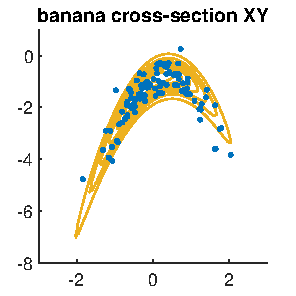
\includegraphics{images/banana3D_sivi_ContourSamples_XY.pdf}
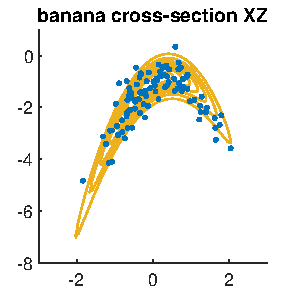
\includegraphics{images/banana3D_sivi_ContourSamples_XZ.pdf}
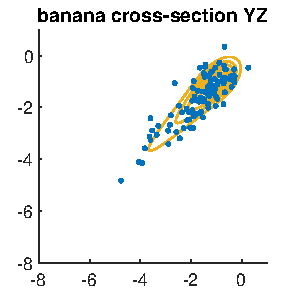
\includegraphics{images/banana3D_sivi_ContourSamples_YZ.pdf}
\caption{Cross-section of the density for a three-dimensional ``banana'' distribution and samples. \todo}
\label{fig:3Dbanana}
\end{figure}

Our experiments with this $d$-dimensional did not return results that we expect. Based on the intuition described in Section~\ref{sec:variance}, we expected the following results:
\begin{enumerate}
\item
As the dimension $d$ increases, the \elbo would be slower to converge and there would be an increase in the variance.
\item
As the number of \mcmc samples $m$ increases, the \elbo variance would decrease.
\end{enumerate}
However, what we found was the following:
\begin{enumerate}
\item
As the dimension $d$ increases, the \elbo converges to a more negative value but the variance otherwise looks stable. \todo imgs
\item
As the number of \mcmc samples $m$ increases, the \elbo variance does not decrease.
\end{enumerate}
We were unable to look into why we obtained these results in time. It may be that the high-dimensional banana distribution is not as difficult to approximate using Gaussians as we expected. We also cannot rule out the possibility of bugs in the code as well. \todo
\\

increasing $K$ in \sivi, variances does not decrease; \uivi performed better even with $m=1$

\todo collect variance?
\\

If more time, look into other high-dimensional synthetic distributions and comparisons to other non-implicit \vi methods.


\subsection{Discussion} \label{sec:discussion}

In this project, we attempted to analyze the theoretical performance of \uivi. Through a simple example, we showed that relying solely on the hierarchical form of the variational distribution is insufficient for obtaining a flexible variational family. We also showed that for a particular choice of the variational conditional and mixing distributions, the variational distribution in \uivi has an equivalent form as a Gaussian convolution. Then under the assumption that the map that transforms the noise is able to learn the inverse CDF of the posterior, we proved that the true posterior distribution is a member of the limiting variational family as the kernel bandwidth goes to zero.
\\

We also attempted to analyze the variance of the \elbo gradient estimator. We discussed the intuition that \uivi can be seen as estimating the \elbo gradient using sampled Gaussian distributions and explained why this may be problematic in high-dimensional problems. We then derived a lower bound of the estimator variance that may be useful if additional assumptions are imposed on the implicit functions. \todo experiments
\\

The work in this project has been mainly exploratory, though a few ideas have been identified that may be of interest for follow-up work. The work by \citet{Plummer:2021} provides an interesting starting point for the theoretical analyses of implicit variational inference methods. While we have applied their approach to show the capacity of the variational family in \uivi as an initial result, the theory can likely be pushed further as discussed in Section~\ref{sec:future:approximation}. In terms of the variance of the \elbo gradient estimator, our result is incomplete and there is still much work to be done. \todo experiments


\newpage


\bibliographystyle{plainnat}
\bibliography{qp}

\end{document}




\subsubsection{\todo to delete}

\todo the results below seem to be leading towards posterior contraction; proposition 2 isn't a result about $q_{\theta,\sigma}(z)$. Theorem 3.1 may still be relevant?

We can further quantify the quality of the approximation by $q_{\theta,\sigma}(z)$ if we make assumptions about the smoothness of $p(z|x)$ and its support. Following \citet{Plummer:2021}, we make the following assumptions.

\begin{assumption} \label{asp:p1}
$\log p(z|x) \in C^\beta([0,1])$. Define $l_j(z_0) = \nabla_z^j\log p(z|x)\big|_{z=z_0}$ for $j=1,\ldots,r$ with $r=\lfloor\beta\rfloor$. For any $\beta>0$, there exists a constant $L>0$ such that for all $z_1\neq z_2$,
\[
|l_r(z_1)-l_r(z_2)| \leq L|z_1-z_2|^{\beta-r} \;.
\]
\end{assumption}

\begin{assumption} \label{asp:p2}
$p(z|x)$ has compact support on $[0,1]$. There exists some interval $[z_1,z_2]\subset[0,1]$ such that $p(z|x)$ is non-decreasing on $[0,z_1]$, non-zero on $[z_1,z_2]$, and non-increasing on $[z_2,1]$.
\end{assumption}

Assumption~\ref{asp:p1} says that the derivatives of $\log p(z|x)$ up to order $r$ are $\beta$-H\"{o}lder continuous, implying that $\log p(z|x)$ is smooth to an extent. The proofs of \citet{Kruijer:2010} and \citet{Plummer:2021} rely heavily on the assumed smoothness in order to ensure that the error between the target distribution and an approximating convolution can be bounded. Assumption~\ref{asp:p2} says that the mass of $p(z|x)$ is concentrated in some compact interval of $z$ and that the tails of $p(z|x)$ outside this interval can be bounded above. This allows the approximation error in the tails to be bounded even as the convolution bandwidth shrinks, and so an analysis of the error only needs to focus on the closed interval in which the mass is concentrated. \citet{Plummer:2021} appear to specify an interval of $[0,1]$ for analytical convenience, whereas the intervals in similar assumptions made by \citet{Ghosal:1999} feature arbitrary finite endpoints.
\\

Under Assumptions~\ref{asp:p1} and \ref{asp:p2}, \citet{Plummer:2021} follow the work of \citet{Kruijer:2010} and consider a sequence of functions $\{p_j\}_{j\geq0}$ constructed through an iterative procedure given by
\begin{align*}
p_{j+1}(z|x) &= p(z|x) - \Delta_\sigma p_j(z|x) \;, \\
\Delta_\sigma p_j(z|x) &= \phi_\sigma * p_j(z|x) - p_j(z|x)
\end{align*}
with $p_0(z|x)=p(z|x)$. The quality of the approximation is then characterized in terms of the error between the convolution \todo

\begin{proposition}
Suppose that $p(z|x)$ satisfies Assumptions~\ref{asp:p1} and \ref{asp:p2} with $\beta\in(2j,2j+2]$. Let $F_{z|x}$ be the cumulative distribution function of the posterior $p(z|x)$. \todo fix this If $\mu_\theta(t)=F_{z|x}^{-1}(t)$ for all $t\in[0,1]$, then
\[
\|\phi_\sigma * p_\beta(z|x) - p(z|x)\|_\infty = O(\sigma^\beta)
\]
with
\[
\phi_\sigma * p_\beta(z|x) = p(z|x)\left(1+O(\sigma^\beta)\left(\sum_{i=1}^rc_i|l_j(z)|^{\frac{\beta}{i}}+c_{r+1}\right)\right)
\]
for non-negative constants $c_i$, $i=1,\ldots,r+1$ and $z\in[0,1]$.
\end{proposition}
\begin{proof}
Suppose that $\mu_\theta(\bft)=F_{\bfz|\bfx}^{-1}(\bft)$ and so $q_\theta(\bfz)=\phi_\sigma*p(\bfz|\bfx)$. Then as $\sigma\rightarrow0$, $q_\theta(\bfz)\rightarrow p(\bfz|\bfx)$.
\end{proof}